
% rubber: module pdftex
\documentclass[english,aspectratio=43,8pt]{beamer}
\usepackage{graphicx}
\usepackage{amssymb}
\usepackage{booktabs}
\usepackage{siunitx}
\usepackage{subcaption}
\usepackage{marvosym}
\usepackage{verbatim}
\usepackage[normalem]{ulem}  % Needed for /sout

\newcommand{\pb}{\si{\pico\barn}}%
\newcommand{\fb}{\si{\femto\barn}}%
\newcommand{\invfb}{\si{\per\femto\barn}}
\newcommand{\GeV}{\si{\giga\electronvolt}}

\hypersetup{colorlinks=true,urlcolor=blue}
\usetheme[]{bjeldbak}


%%% For wider frames
\newcommand\Wider[2][3em]{%
\makebox[\linewidth][c]{%
  \begin{minipage}{\dimexpr\textwidth+#1\relax}
  \raggedright#2
  \end{minipage}%
  }%
}
%%% For wider frames end

\newcommand{\backupbegin}{%
   \newcounter{finalframe}
   \setcounter{finalframe}{\value{framenumber}}
}
\newcommand{\backupend}{%
   \setcounter{framenumber}{\value{finalframe}}
}

\newcommand\blfootnote[1]{%
  \begingroup
  \renewcommand\thefootnote{}\footnote{#1}%
  \addtocounter{footnote}{-1}%
  \endgroup
}

\begin{document}

\title{Gantry Electronics Hub Box}
\author[C. Fangmeier]{\textbf{Caleb Fangmeier}, Frank Golf, Ilya Kravchenko, Shubhanshu Chauhan, Changwoo Joo}
\institute[UNL]{University of Nebraska \-- Lincoln}
\date{TFPX General Metting | Jan 24, 2020}

\titlegraphic{%
\begin{figure}
  
\includegraphics[width=1in]{CMSlogo.png}\hspace{0.75in}
\includegraphics[width=1in]{nebraska-n.png}
\end{figure}
}

\begin{frame}[plain]
  \titlepage%
\end{frame}

\begin{frame}{Introduction}
      \begin{itemize}
          \item Module construction will involve the use of systems based around the Aerotech AGS10000 Gantry
          \item The system includes components that must be wired together
          \item Phase I solutions worked, but were not robust or flexible
          \item Propose a "hub box" that manages the interconnects
      \end{itemize}
      \begin{figure}
        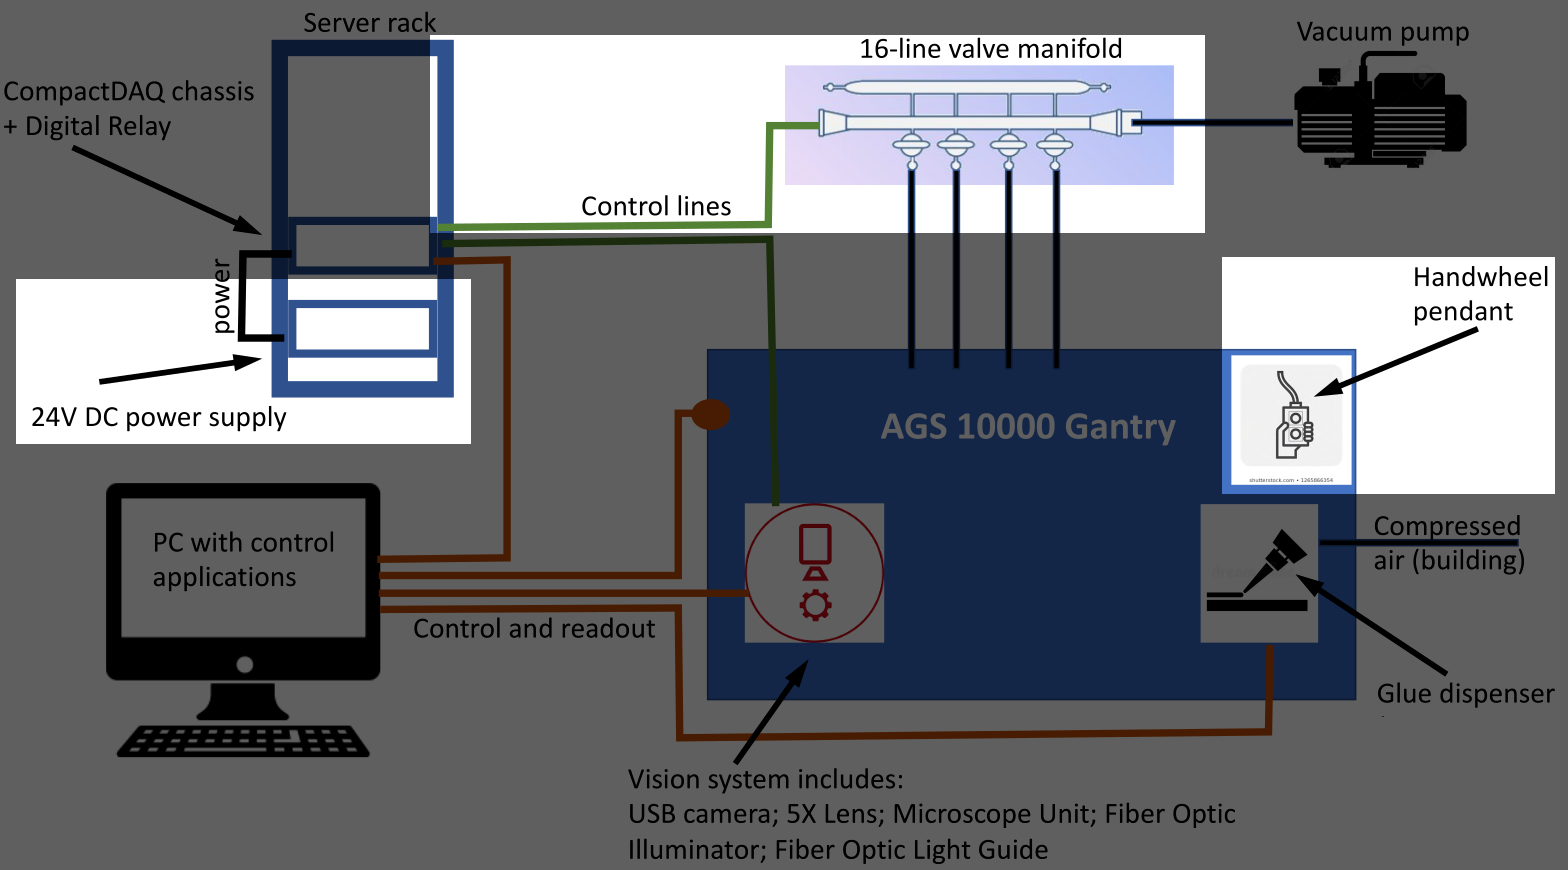
\includegraphics[width=\textwidth]{figures/gantry_schematic.png}
      \end{figure}
\end{frame}


\begin{frame}{Gantry Electronics Overview}
    \begin{figure}
        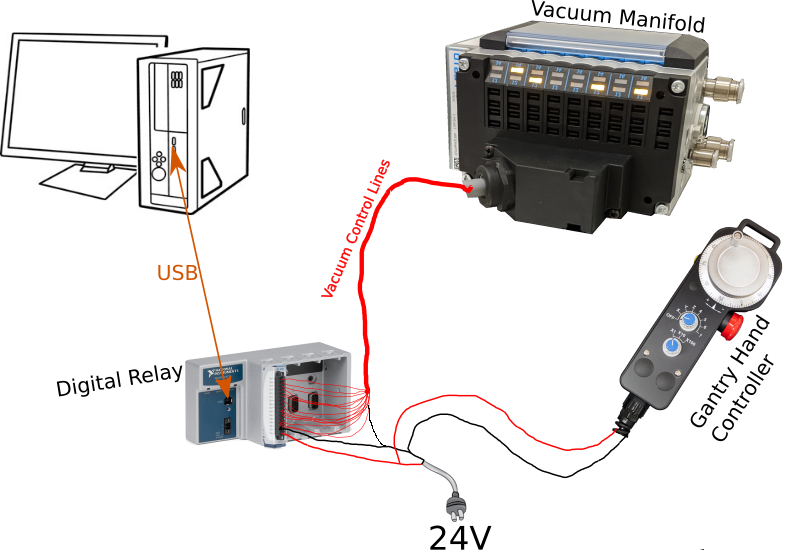
\includegraphics[width=\textwidth]{figures/gantry_aux_electronics.png}
    \end{figure}
\end{frame}

\begin{frame}{Gantry Hub Box}
  \begin{columns}
  \begin{column}{0.3\textwidth}
    {\large Features:}
    \begin{itemize}
      \item Switch with indicator light
      \item Safety fuse
      \item Standard AC power plug
      \item Integrated 24V Supply
      \item 6 pairs of 24V bananna plugs
      \item (back side) D-sub style connectors for manifold hookups
        \begin{itemize}
          \item Can support two 16-channel manifolds.
        \end{itemize}
    \end{itemize}
  \end{column}
  \begin{column}{0.7\textwidth}
    \begin{figure}
        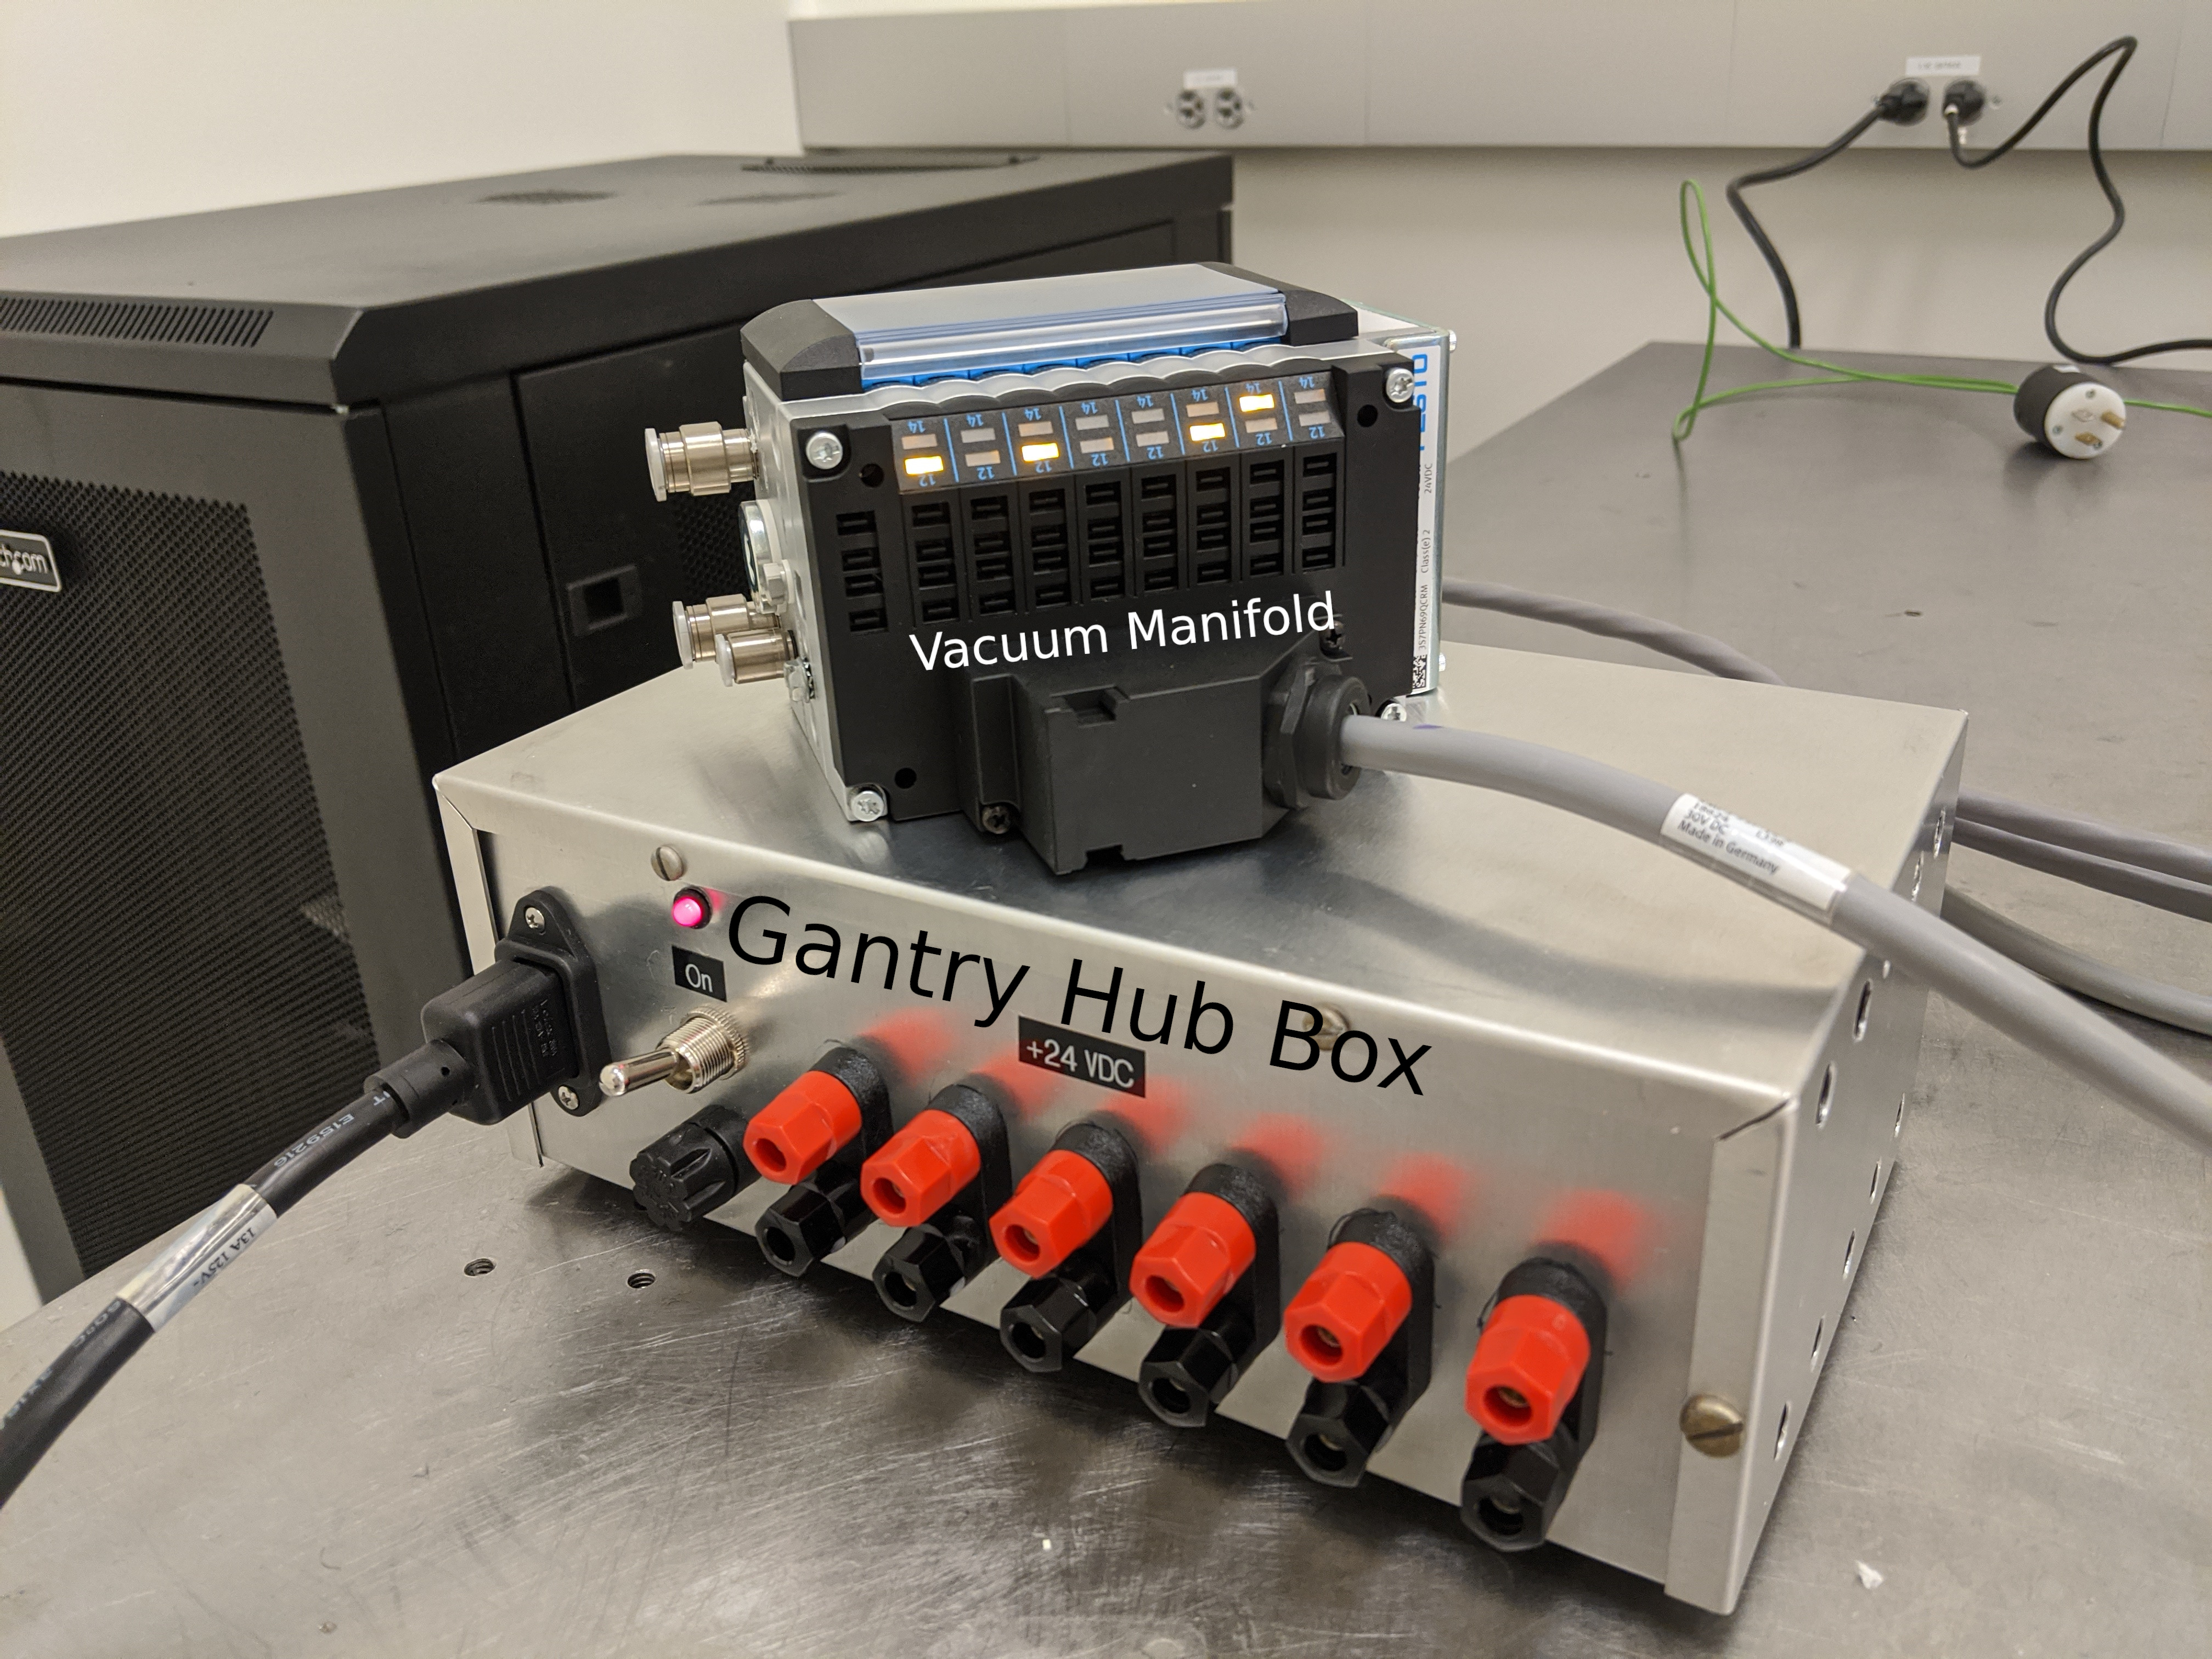
\includegraphics[width=\textwidth]{figures/gantry_hub_action.jpg}
    \end{figure}
  \end{column}
  \end{columns}
\end{frame}

\begin{frame}{Gantry Hub Box cont.}
  \begin{columns}
  \begin{column}{0.5\textwidth}
    {\large Interior}
    \begin{figure}
        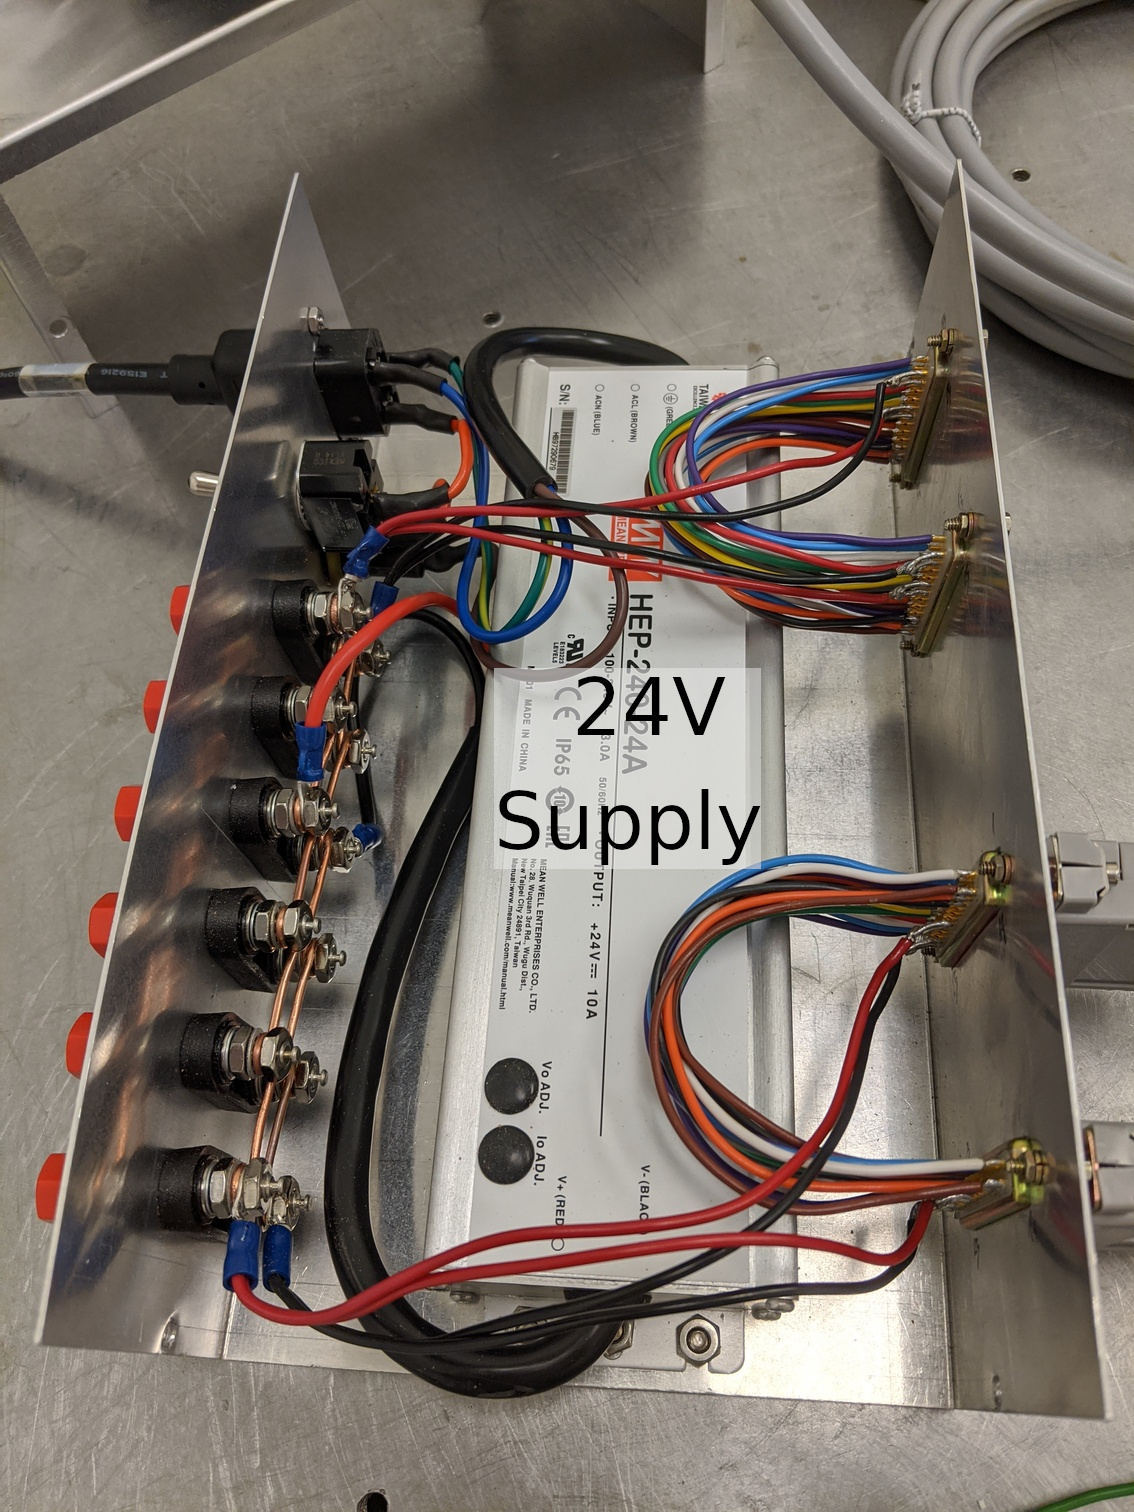
\includegraphics[width=\textwidth]{figures/gantry_hub_interior.jpg}
    \end{figure}
  \end{column}
  \begin{column}{0.5\textwidth}
    {\large Rear View}
    \begin{figure}
        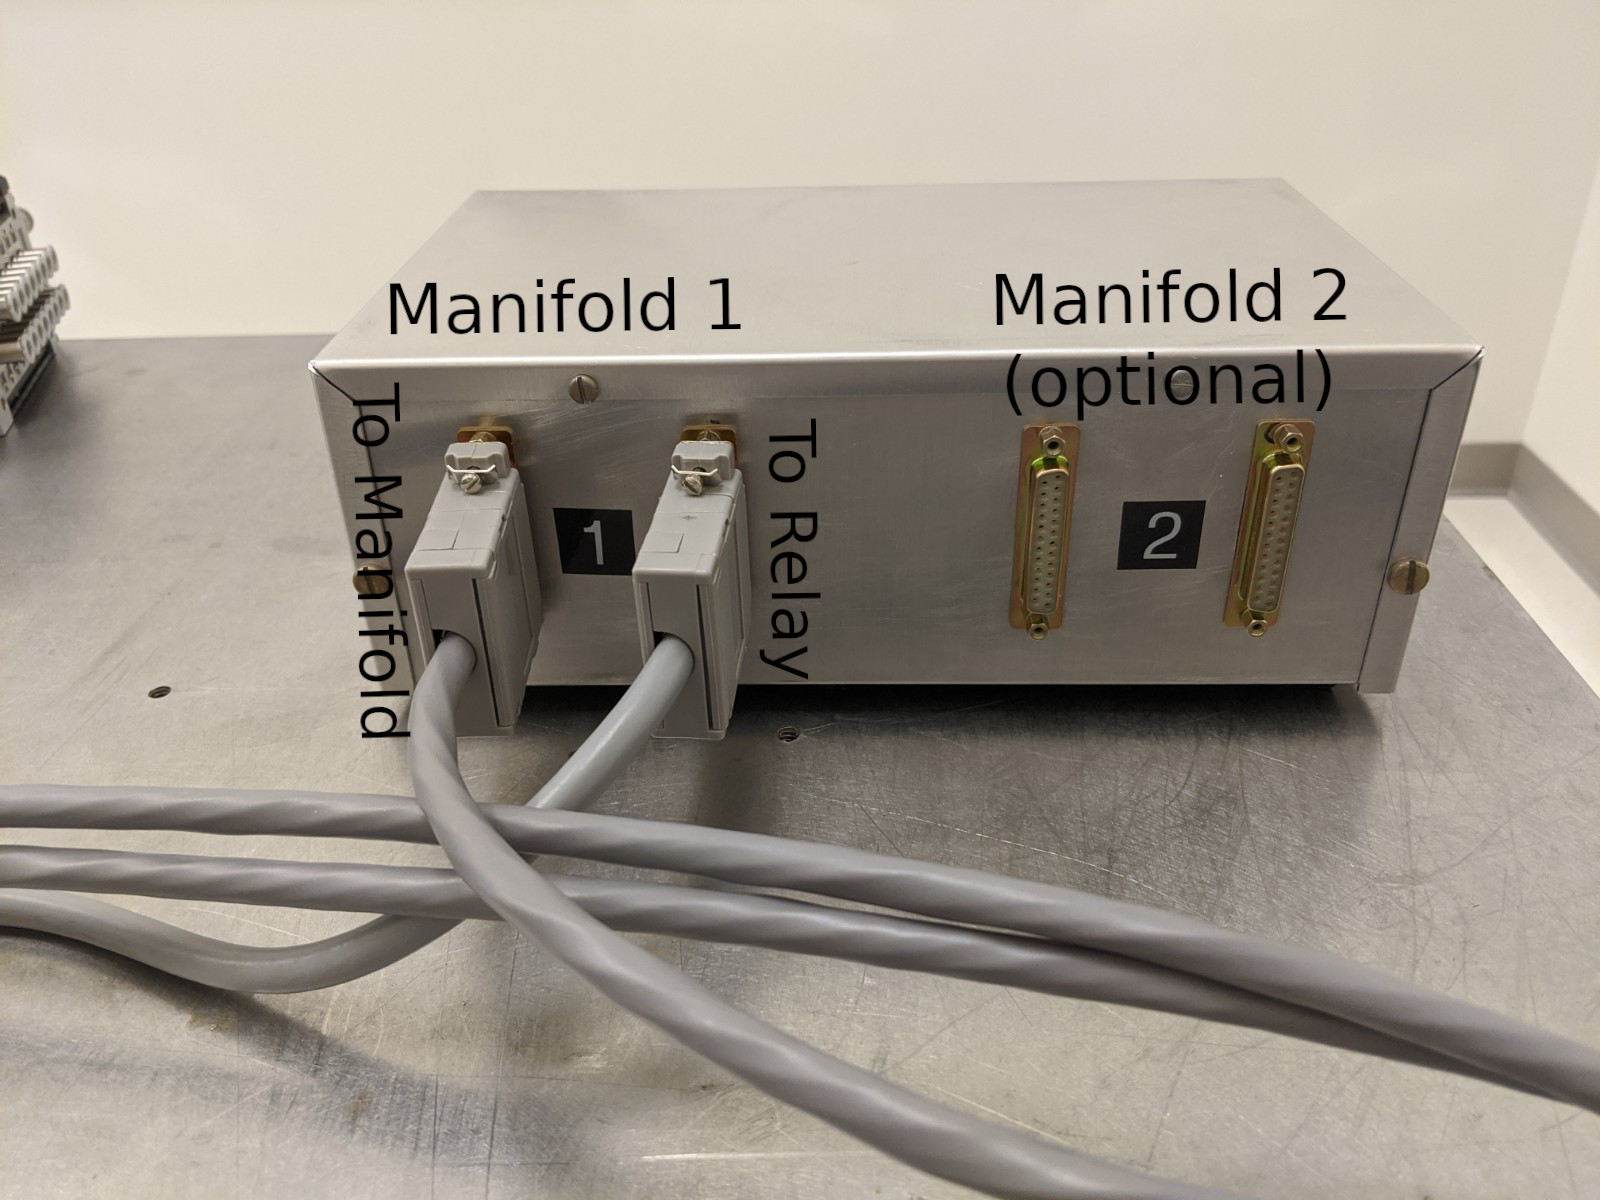
\includegraphics[width=\textwidth]{figures/gantry_hub_rear.jpg}
    \end{figure}
  \begin{itemize}
    \item UNL can build similar boxes for other gantry sites
    \item Cost including parts and labor is roughly \$1000.
    \item Can also share designs if sites would prefer to build themselves.
  \end{itemize}
  \end{column}
  \end{columns}
\end{frame}


\appendix
\backupbegin%

\begin{frame}
  \begin{center}
    {\Huge BACKUP}
  \end{center}
\end{frame}

\begin{frame}{Gantry System Overview}
    \begin{figure}
        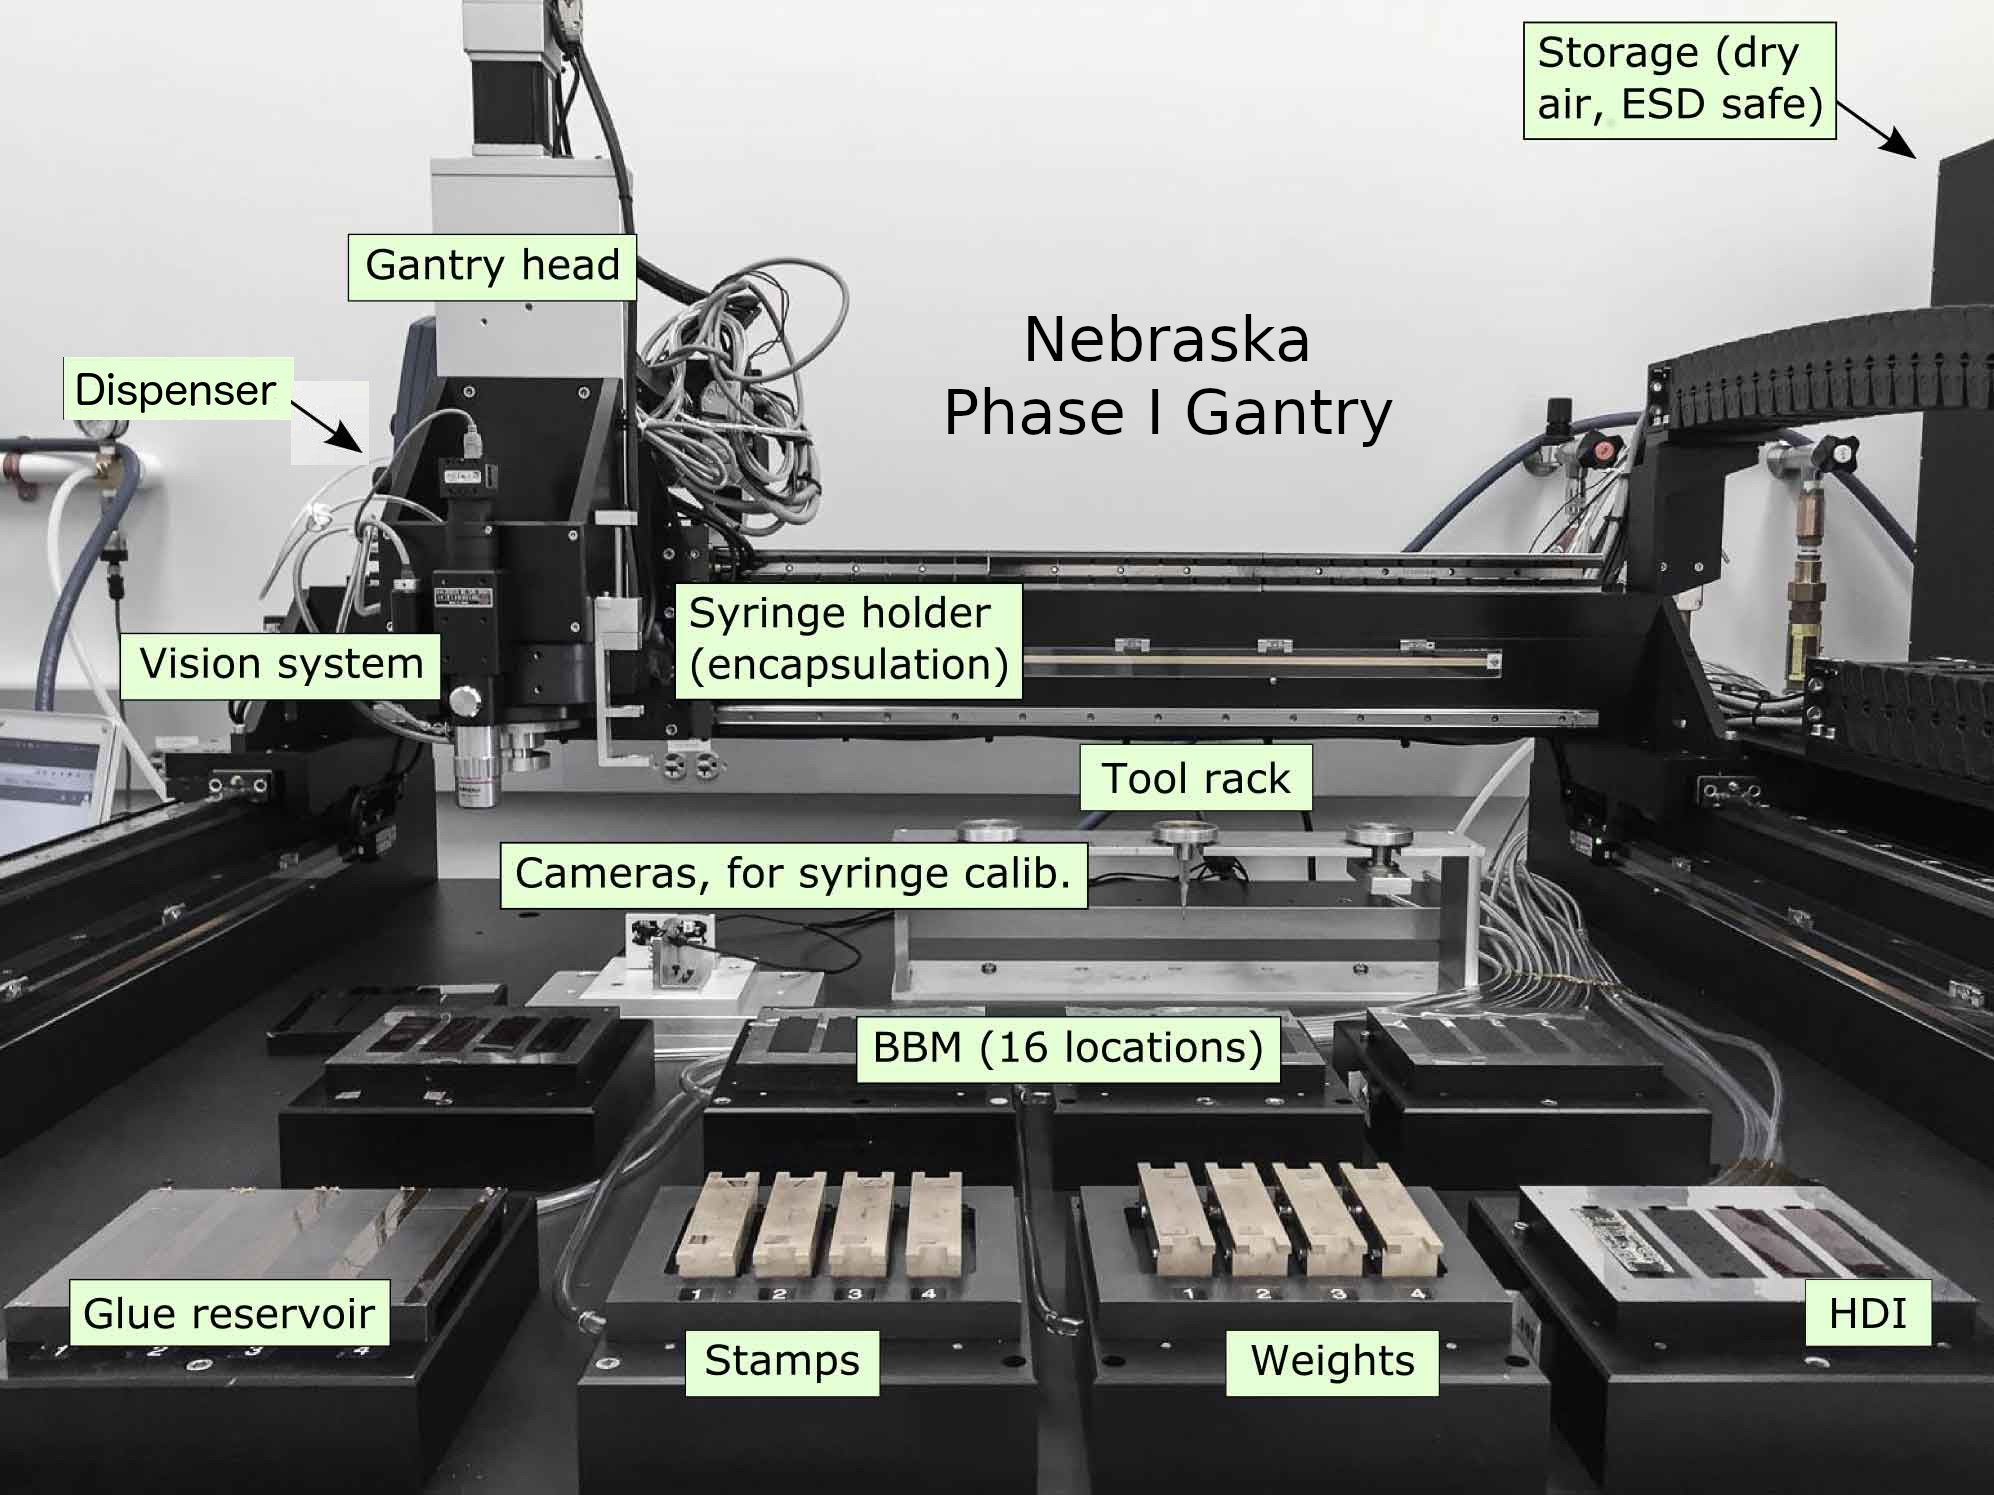
\includegraphics[width=\textwidth]{figures/gantry.png}
    \end{figure}
\end{frame}


% \backupend%

\end{document}
